% Options for packages loaded elsewhere
\PassOptionsToPackage{unicode}{hyperref}
\PassOptionsToPackage{hyphens}{url}
%
\documentclass[
]{article}
\usepackage{lmodern}
\usepackage{amssymb,amsmath}
\usepackage{ifxetex,ifluatex}
\ifnum 0\ifxetex 1\fi\ifluatex 1\fi=0 % if pdftex
  \usepackage[T1]{fontenc}
  \usepackage[utf8]{inputenc}
  \usepackage{textcomp} % provide euro and other symbols
\else % if luatex or xetex
  \usepackage{unicode-math}
  \defaultfontfeatures{Scale=MatchLowercase}
  \defaultfontfeatures[\rmfamily]{Ligatures=TeX,Scale=1}
\fi
% Use upquote if available, for straight quotes in verbatim environments
\IfFileExists{upquote.sty}{\usepackage{upquote}}{}
\IfFileExists{microtype.sty}{% use microtype if available
  \usepackage[]{microtype}
  \UseMicrotypeSet[protrusion]{basicmath} % disable protrusion for tt fonts
}{}
\makeatletter
\@ifundefined{KOMAClassName}{% if non-KOMA class
  \IfFileExists{parskip.sty}{%
    \usepackage{parskip}
  }{% else
    \setlength{\parindent}{0pt}
    \setlength{\parskip}{6pt plus 2pt minus 1pt}}
}{% if KOMA class
  \KOMAoptions{parskip=half}}
\makeatother
\usepackage{xcolor}
\IfFileExists{xurl.sty}{\usepackage{xurl}}{} % add URL line breaks if available
\IfFileExists{bookmark.sty}{\usepackage{bookmark}}{\usepackage{hyperref}}
\hypersetup{
  pdftitle={Wypadki drogowe w Polsce na tle statystyk Unii Europejskiej},
  pdfauthor={Karol Jaroń, Maciej Karczewski, Wojciech Smolak},
  hidelinks,
  pdfcreator={LaTeX via pandoc}}
\urlstyle{same} % disable monospaced font for URLs
\usepackage[margin=1in]{geometry}
\usepackage{graphicx,grffile}
\makeatletter
\def\maxwidth{\ifdim\Gin@nat@width>\linewidth\linewidth\else\Gin@nat@width\fi}
\def\maxheight{\ifdim\Gin@nat@height>\textheight\textheight\else\Gin@nat@height\fi}
\makeatother
% Scale images if necessary, so that they will not overflow the page
% margins by default, and it is still possible to overwrite the defaults
% using explicit options in \includegraphics[width, height, ...]{}
\setkeys{Gin}{width=\maxwidth,height=\maxheight,keepaspectratio}
% Set default figure placement to htbp
\makeatletter
\def\fps@figure{htbp}
\makeatother
\setlength{\emergencystretch}{3em} % prevent overfull lines
\providecommand{\tightlist}{%
  \setlength{\itemsep}{0pt}\setlength{\parskip}{0pt}}
\setcounter{secnumdepth}{-\maxdimen} % remove section numbering

\title{Wypadki drogowe w Polsce na tle statystyk Unii Europejskiej}
\author{Karol Jaroń, Maciej Karczewski, Wojciech Smolak}
\date{18 06 2020}

\begin{document}
\maketitle

\hypertarget{wprowadzenie}{%
\section{Wprowadzenie}\label{wprowadzenie}}

W raporcie zebrano oraz przedstawiono dane dotyczace śmiertelnych
wypadków drogowych, z podziałem na państwa UE. Przedstawiono również
statystykę na temat liczby pojazdów w krajach UE. Wyniki analizowane są
po kątem tego, jak na tle reszty państw wspólnoty wypada Polska.
Podstawowym źródłem danych jest agencja Eurostat. W drugiej części
raportu przedstawiono szczegółowe dane dla Polski w rozbiciu na powiaty.
Źródłem danych był Bank Danych Lokalnych GUS.

\hypertarget{dane-unia-europejska}{%
\section{Dane Unia Europejska}\label{dane-unia-europejska}}

\hypertarget{zabici-oguxf3ux142em-w-wypadkach-drogowych-w-paux144stwach-ue-2018}{%
\subsection{Zabici ogółem w wypadkach drogowych w państwach UE
(2018)}\label{zabici-oguxf3ux142em-w-wypadkach-drogowych-w-paux144stwach-ue-2018}}

Dane za rok 2018 (z wyłączeniem Turcji) obejmują łączną liczbę zabitych
oraz wartość przeliczoną na 100 tys. mieszkańców.

Poniższe wykresy pokazują, że Polska przoduje w unijnych statystykach
dot. ofiar śmiertlenych wypadków drogowych. Dotyczy to zarówno wartości
bezwględnych, jak liczby wypadków na 100 tys. mieszkańców.

\begin{figure}

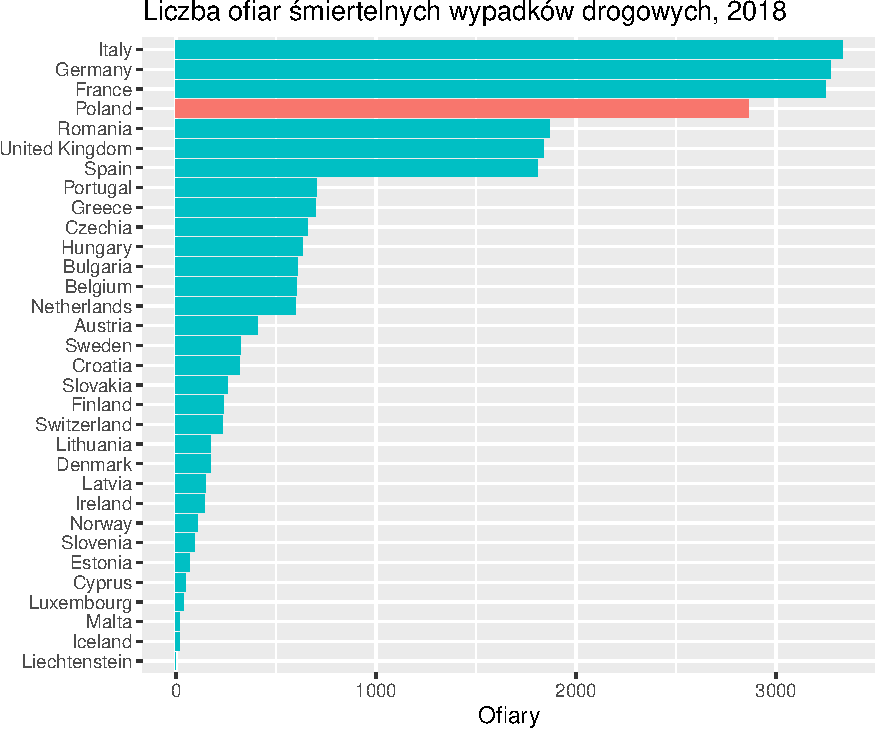
\includegraphics{raport_wypadki_files/figure-latex/unnamed-chunk-2-1} \hfill{}

\caption{Wykres 1.}\label{fig:unnamed-chunk-2}
\end{figure}

\begin{figure}

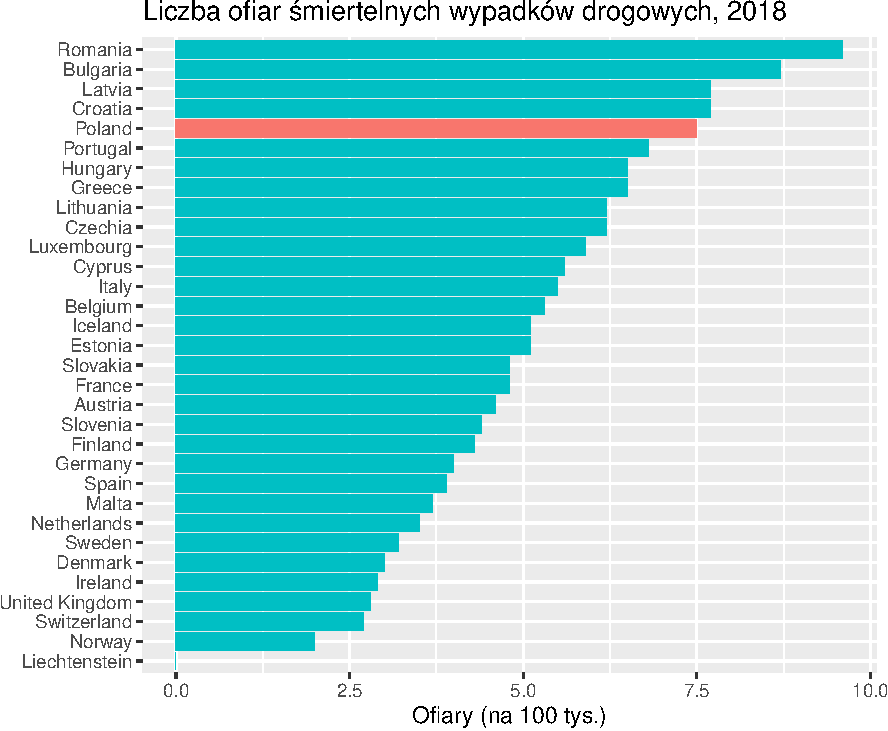
\includegraphics{raport_wypadki_files/figure-latex/unnamed-chunk-3-1} \hfill{}

\caption{Wykres 2.}\label{fig:unnamed-chunk-3}
\end{figure}

\hypertarget{zabici-w-wypadkach-drogowych-w-paux144stwach-ue-w-ujux119ciu-geograficznym-2018}{%
\subsection{Zabici w wypadkach drogowych w państwach UE w ujęciu
geograficznym
(2018)}\label{zabici-w-wypadkach-drogowych-w-paux144stwach-ue-w-ujux119ciu-geograficznym-2018}}

Dane dot. współczynnika śmiertelności w wypadkach drogowych (na 100
tys.) zostały podzielone na 4 przedziały i zestawione z informacją
geograniczną Eurostat.

Poniższa mapa pokazuje, że najgorsza sytuacja pod względem ofiar
śmiertelnych wypadków drogowych panuje w państwa Europy
Środkowo-Wschodniej oraz na Bałkanach.

\begin{figure}

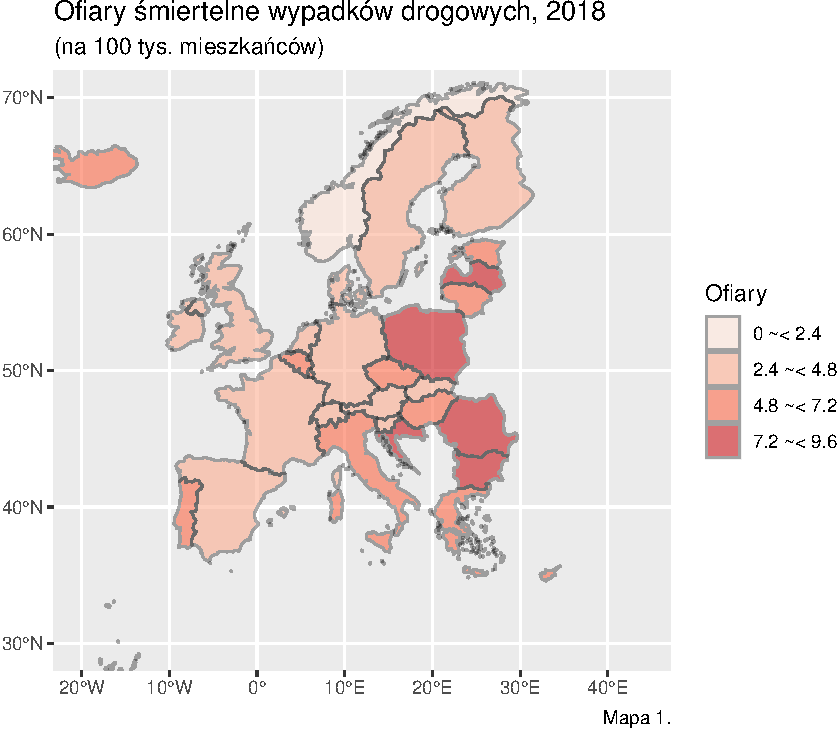
\includegraphics{raport_wypadki_files/figure-latex/unnamed-chunk-5-1} \hfill{}

\caption{Mapa 1.}\label{fig:unnamed-chunk-5}
\end{figure}

Wniosek ten ptwierdza mapa, na którą naniesiono dane w skali dyskretnej.

\begin{figure}

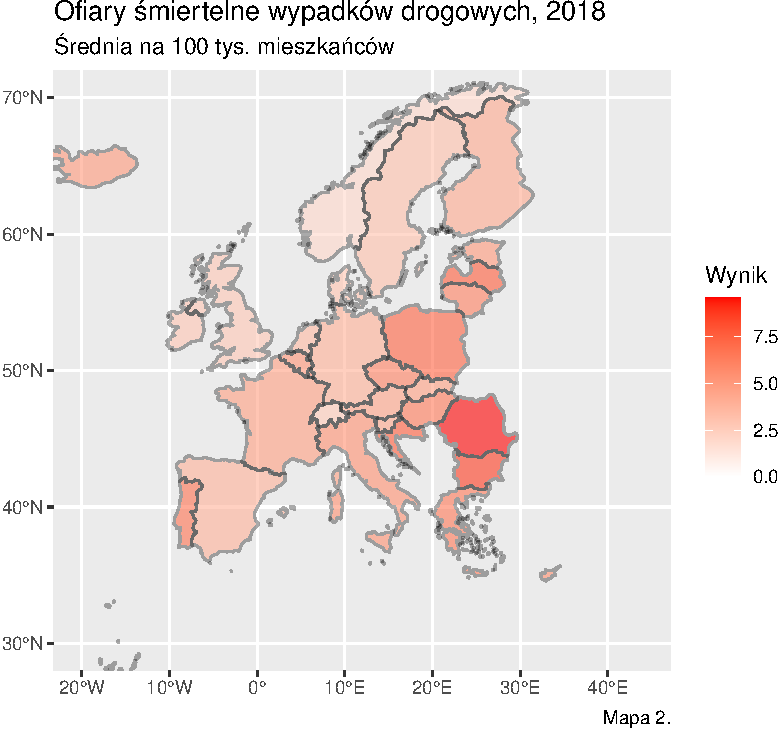
\includegraphics{raport_wypadki_files/figure-latex/unnamed-chunk-6-1} \hfill{}

\caption{Mapa 2.}\label{fig:unnamed-chunk-6}
\end{figure}

\hypertarget{zabici-w-wypadkach-drogowych-w-paux144stwach-ue-wg-pojazdu-2017}{%
\subsection{Zabici w wypadkach drogowych w państwach UE wg pojazdu
(2017)}\label{zabici-w-wypadkach-drogowych-w-paux144stwach-ue-wg-pojazdu-2017}}

Dane Eurostat wymagają przeliczenia w stosunku do rozmiaru populacji w
celu uzyskania miarodajnego porównania sytuacji w poszczególnych
państwach.

Poniższy wykres wskazuje, że Polska jest jednym liderów pod względem
liczby ofiar śmiertelnych wypadków drogowych z udziałem samochodów
osobowych.

\begin{figure}

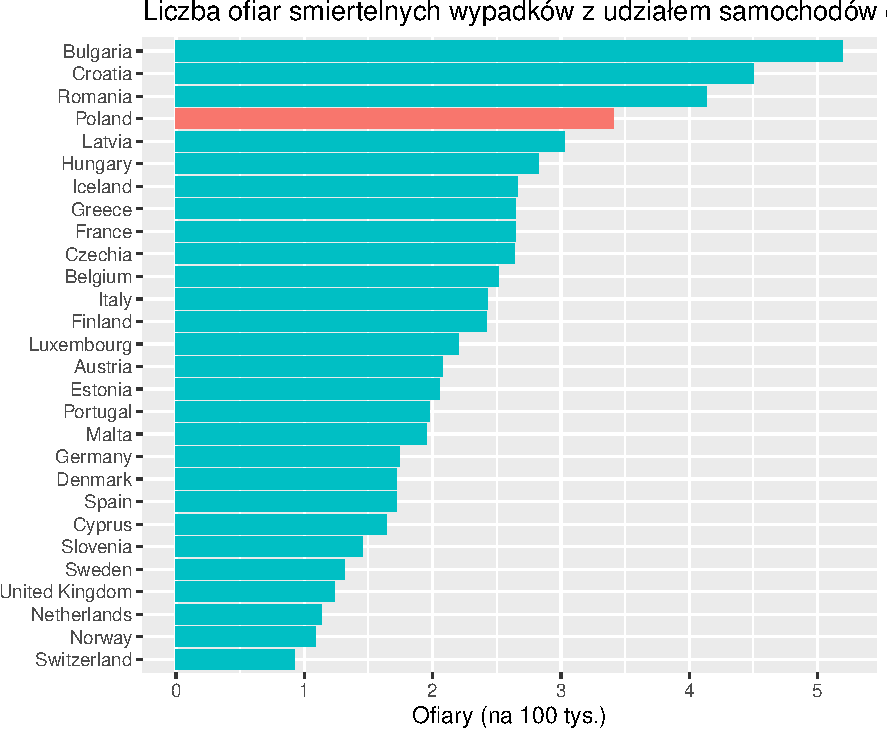
\includegraphics{raport_wypadki_files/figure-latex/unnamed-chunk-8-1} \hfill{}

\caption{Wykres 3.}\label{fig:unnamed-chunk-8}
\end{figure}

Polska nieco lepiej wypadła pod względem, liczby ofiar śmiertlenych
wypadków z udziałem rowerzystów. Polska ustępuje pod tym względem
niektórym państwom Europy Zachodniej, w tym Holandii (państwo o
najwyśzym odsetku rowerzystów w Europie).

\begin{figure}

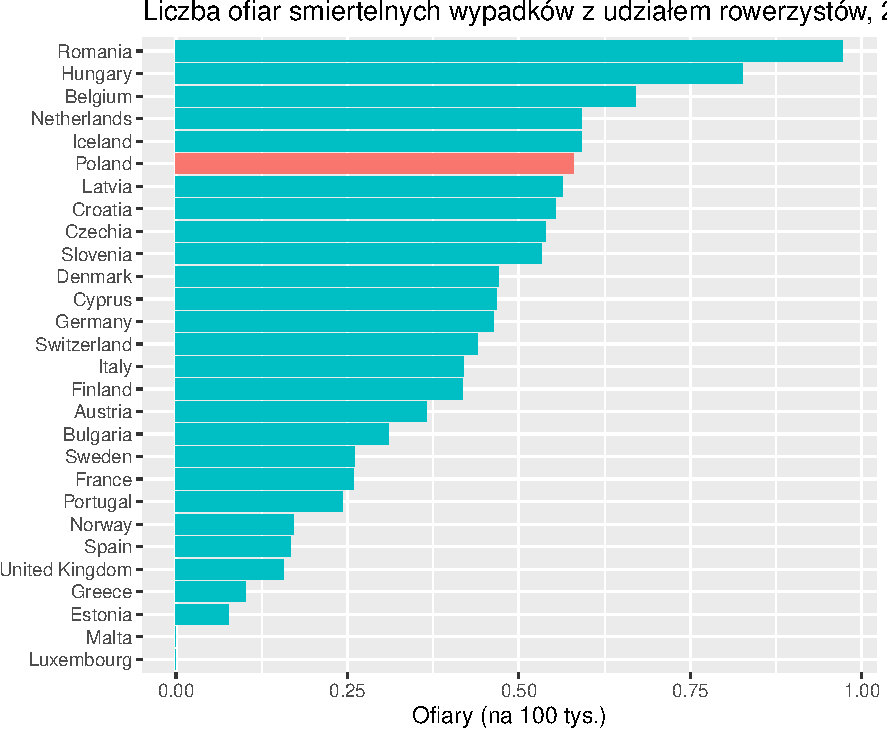
\includegraphics{raport_wypadki_files/figure-latex/unnamed-chunk-9-1} \hfill{}

\caption{Wykres 4.}\label{fig:unnamed-chunk-9}
\end{figure}

Niestety w zasobach Eurostat brakuje danych dotyczących ofiar wypadków z
udziałem innych typów pojazdów, w tym pojazdów transportowych lub
motocykli.

\hypertarget{ofiary-wypadkuxf3w-z-podziaux142em-na-uux17cytkownikuxf3w-druxf3g-2017}{%
\subsection{Ofiary wypadków z podziałem na użytkowników dróg
(2017)}\label{ofiary-wypadkuxf3w-z-podziaux142em-na-uux17cytkownikuxf3w-druxf3g-2017}}

Dane za rok 2017 zostały przeliczone w stosunku do rozmiaru populacji.

Zgodnie z danymi Polska przoduje pod względem liczby ofiar śmiertlenych
wypadków wśród pieszych uczestników ruchu, co obrazuje Wykres 5.

\begin{figure}

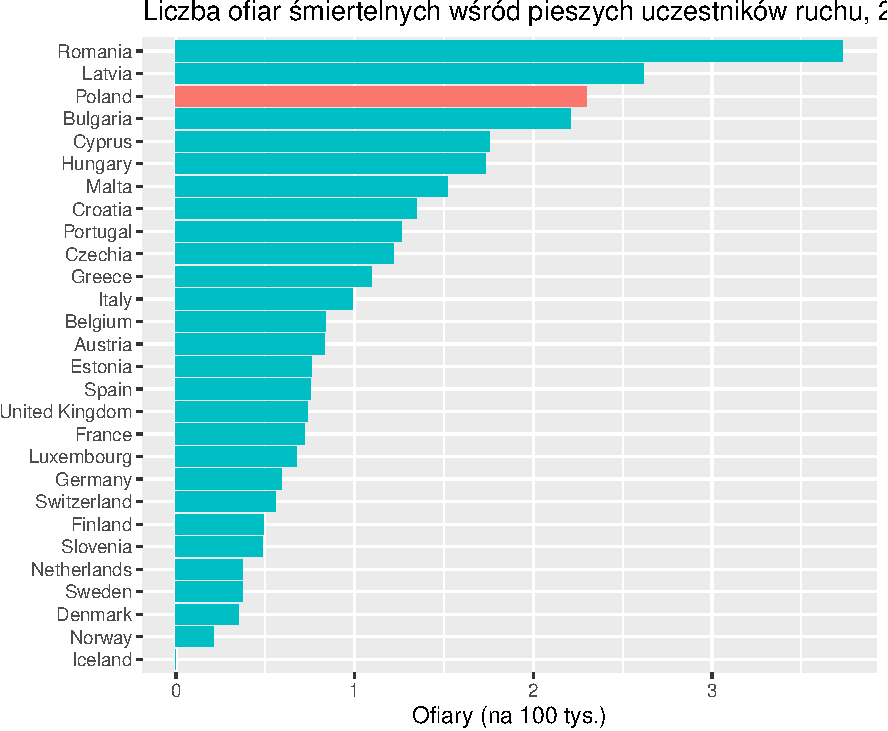
\includegraphics{raport_wypadki_files/figure-latex/unnamed-chunk-11-1} \hfill{}

\caption{Wykres 5.}\label{fig:unnamed-chunk-11}
\end{figure}

Sytuacja jest niewiele lepsza pod względem ofiar śmiertelnych wśród
pasażerów pojazdów mechanicznych (wykres 6).

\begin{figure}

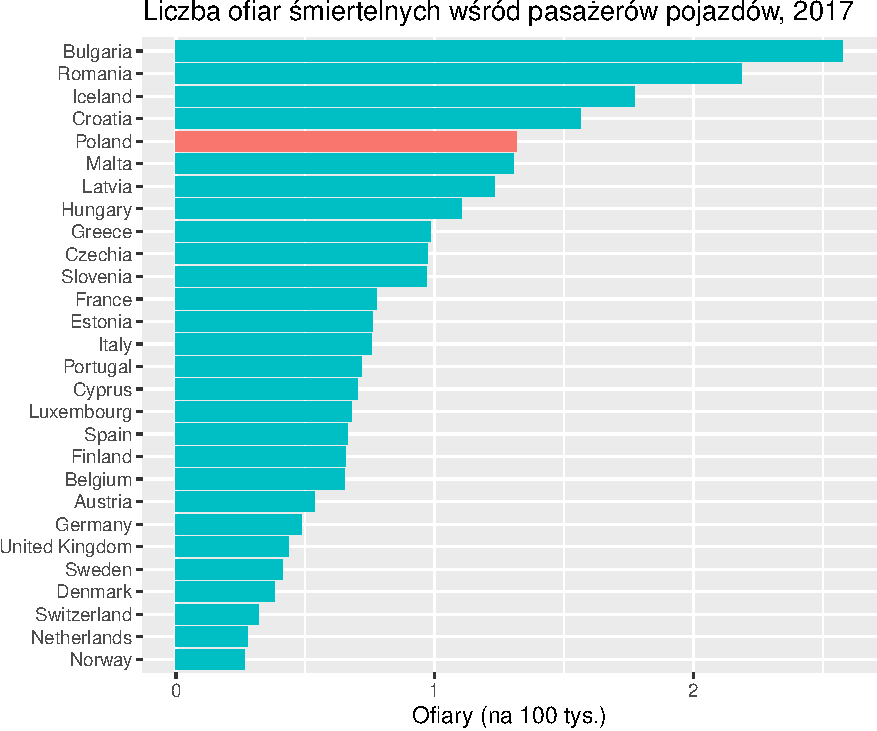
\includegraphics{raport_wypadki_files/figure-latex/unnamed-chunk-12-1} \hfill{}

\caption{Wykres 6.}\label{fig:unnamed-chunk-12}
\end{figure}

Jeśli chodzi o odsetek ofiar wypadków drogowych Wsród kierujących
pojazdami, Polskę wyprzedzają pod tym względem niektóre państwa Europy
Zachodniej (wykres 7).

\begin{figure}

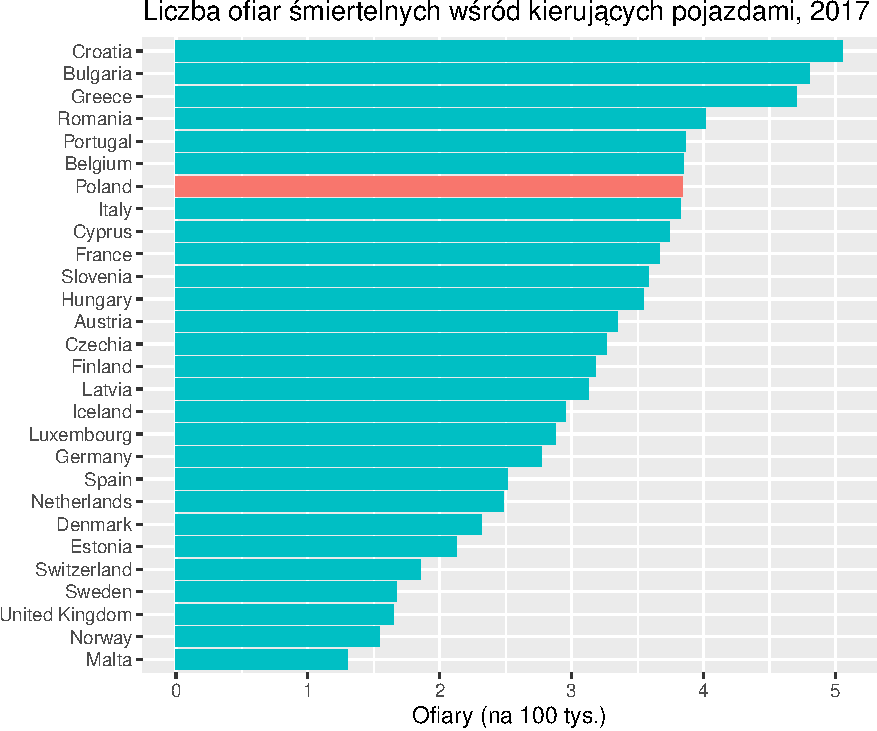
\includegraphics{raport_wypadki_files/figure-latex/unnamed-chunk-13-1} \hfill{}

\caption{Wykres 7.}\label{fig:unnamed-chunk-13}
\end{figure}

\hypertarget{ofiary-wypadkuxf3w-wg-rodzaju-infrastruktury-drogowej}{%
\subsection{Ofiary wypadków wg rodzaju infrastruktury
drogowej}\label{ofiary-wypadkuxf3w-wg-rodzaju-infrastruktury-drogowej}}

Dane za rok 2017 zostały przeliczone w stosunku do rozmiaru populacji.

Pod względem liczby ofiar śmiertelnych wypadków drogowych na
autostradach (w przeliczeniu na 100 tys. mieszkańców), Polska plasuje
dole rankingu państw UE (wykres 8). Może to jednak wynikać z faktu, iż
długość sieci autostrad w Polsce pozostaje nadal relatywnie mała.

\begin{figure}

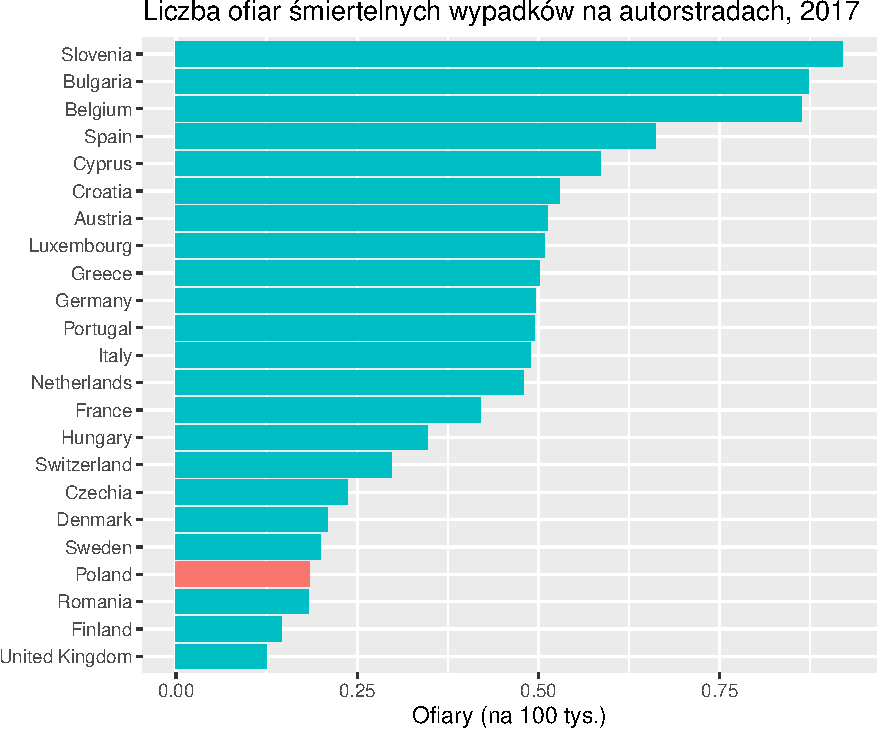
\includegraphics{raport_wypadki_files/figure-latex/unnamed-chunk-15-1} \hfill{}

\caption{Wykres 8.}\label{fig:unnamed-chunk-15}
\end{figure}

W celu weryfikacji tej hipotezy, należy przeliczyć średnią liczbę ofiar
śmiertlenych wypadków drogowych na autostradach na tysiąc km dróg tego
rodzaju.

Choć dane Eurostatu nt. stanu infrastruktury drogowej za 2017 r. są
niestety niepełne, to nadal obrazują różnicę między Polską a państwa
Europy Zachodniej. Pod względem średniej liczby ofiar śmiertelnych
wypadków drogowych na autostradach w przeliczenia na 1 tys. km tego
rodzaju dróg, Polska plasuje się w na trzecim miejscu (za Bułgarią i
Rumunią).

\begin{figure}

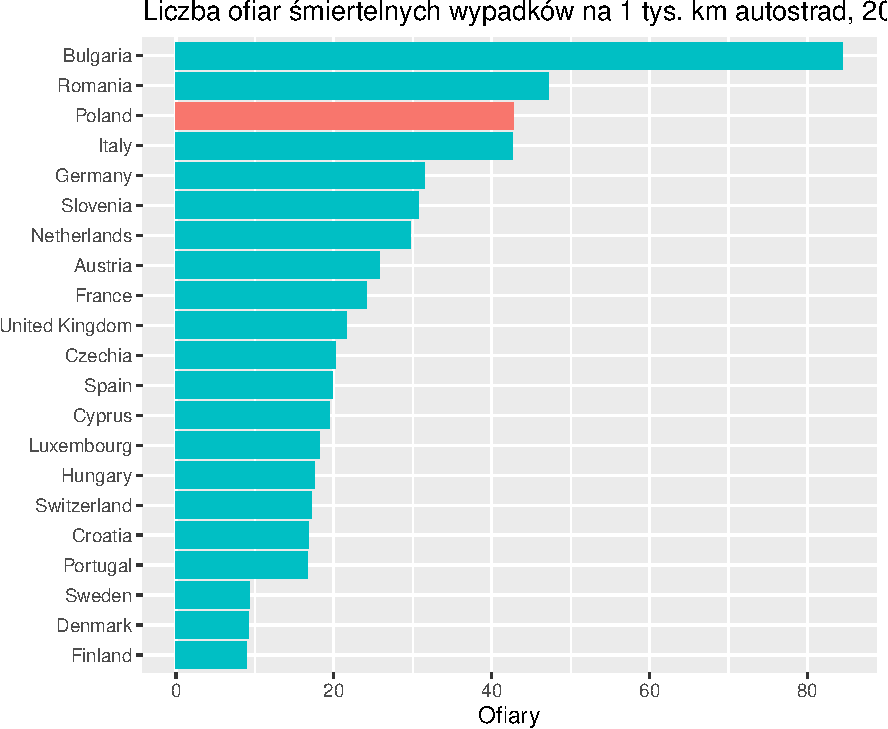
\includegraphics{raport_wypadki_files/figure-latex/unnamed-chunk-17-1} \hfill{}

\caption{Wykres 9.}\label{fig:unnamed-chunk-17}
\end{figure}

Na wykresach 10 i 11 przestawiono dane dot. średniej liczby ofiar
wypadków na drogach ulokowanych na obszarze zabudowanym oraz na drogach
wiejskich (w przeliczeniu na 100 tys. mieszkańców). Również i w tych
zestawieniach Polska osiąga wysokie miejsca.

\begin{figure}

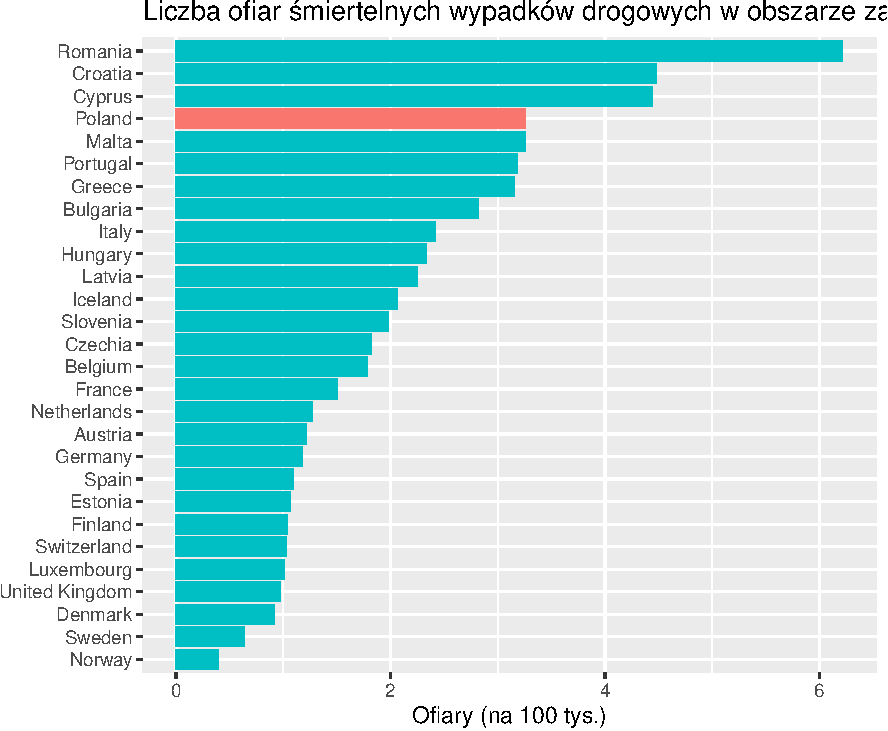
\includegraphics{raport_wypadki_files/figure-latex/unnamed-chunk-18-1} \hfill{}

\caption{Wykres 10.}\label{fig:unnamed-chunk-18}
\end{figure}

\begin{figure}

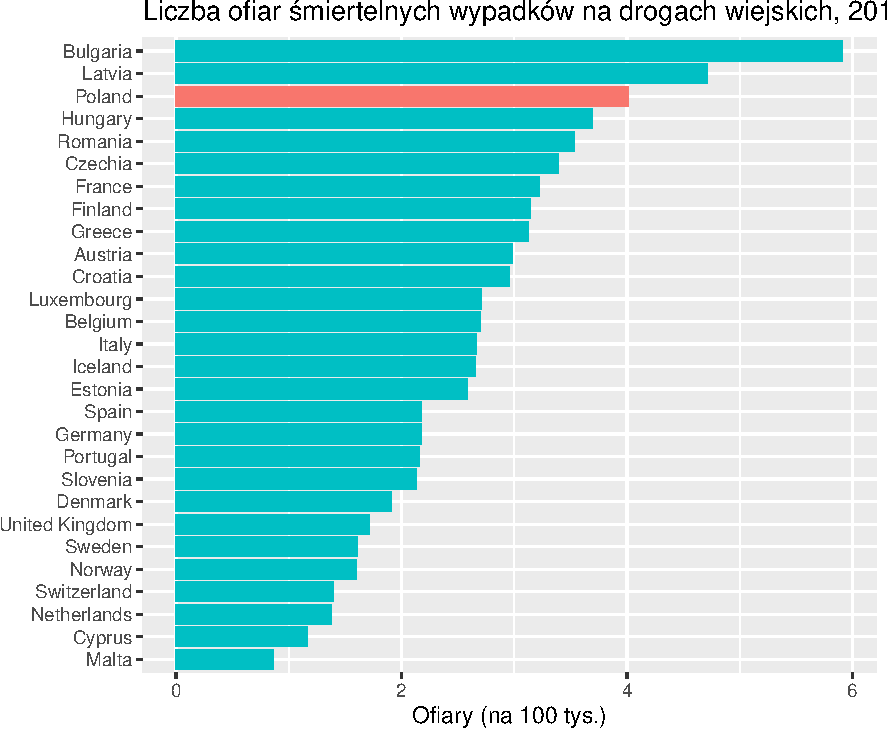
\includegraphics{raport_wypadki_files/figure-latex/unnamed-chunk-19-1} \hfill{}

\caption{Wykres 11.}\label{fig:unnamed-chunk-19}
\end{figure}

\hypertarget{ofiary-ux15bmiertelne-wypadkuxf3w-drogowych-w-latach-2000-2018-w-wybranych-paux144stwach-ue---analiza-trendu}{%
\subsection{Ofiary śmiertelne wypadków drogowych w latach 2000-2018 w
wybranych państwach UE - analiza
trendu}\label{ofiary-ux15bmiertelne-wypadkuxf3w-drogowych-w-latach-2000-2018-w-wybranych-paux144stwach-ue---analiza-trendu}}

Dane za lata 2000-2018 obejmuję jedynie wybrane państwa UE: Polskę,
Niemcy, Francję, Wielką Brytanię (stan na 2018 r.), Hiszpanię, Szwecję,
Włochy, Austrię, Belgię i Portugalię.

Wykres 12 potwierdza trend spadkowy dla liczba ofiar wypadków rogowych
(w przeliczeniu na 100 tys.) mieszkańców we wszystkich przytoczonych
państwawch. Dotyczy to również Polski, która jedynie w latach 2000-2003
notowała mniej ofiar śmiertelnych niż Portugalia.

\begin{figure}

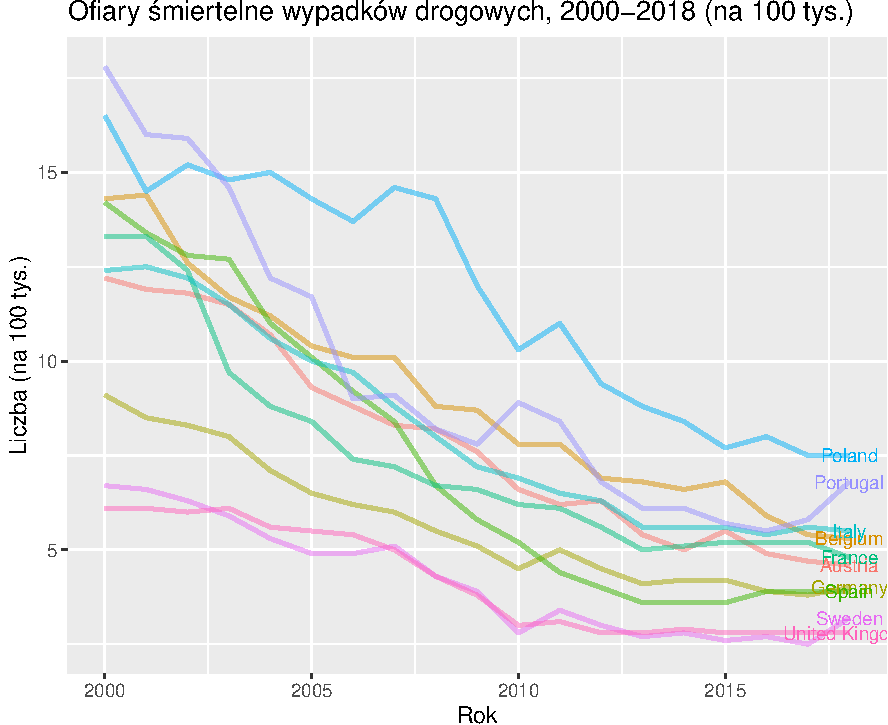
\includegraphics{raport_wypadki_files/figure-latex/unnamed-chunk-21-1} \hfill{}

\caption{Wykres 12.}\label{fig:unnamed-chunk-21}
\end{figure}

\hypertarget{ofiary-ux15bmiertelne-wypadkuxf3wdrogowych-na-poziomie-jednostek-nuts-2-2018-r.}{%
\subsection{ofiary śmiertelne wypadkówdrogowych na poziomie jednostek
NUTS-2 (2018
r.)}\label{ofiary-ux15bmiertelne-wypadkuxf3wdrogowych-na-poziomie-jednostek-nuts-2-2018-r.}}

Dane oraz informacje geoprzestrzenne pochodzą z zasobów agencji
Eurostat. W analizie pominięto regiony ulokowane na obszarze Turcji.
Wyniki podzielono w oparciu o pięć przedziałów.

Dane dot. liczby ofiar śmiertelnych wypadków drogowych (w przeliczeniu
na 1 mln mieszkańców) na poziomie regionów NUTS-2, wyraźnie wskazują, że
obszary o najwyśzym współczynniku wypadkowości znajdują się na
wschodnich rubieżach UE (mapa 3).

\begin{figure}

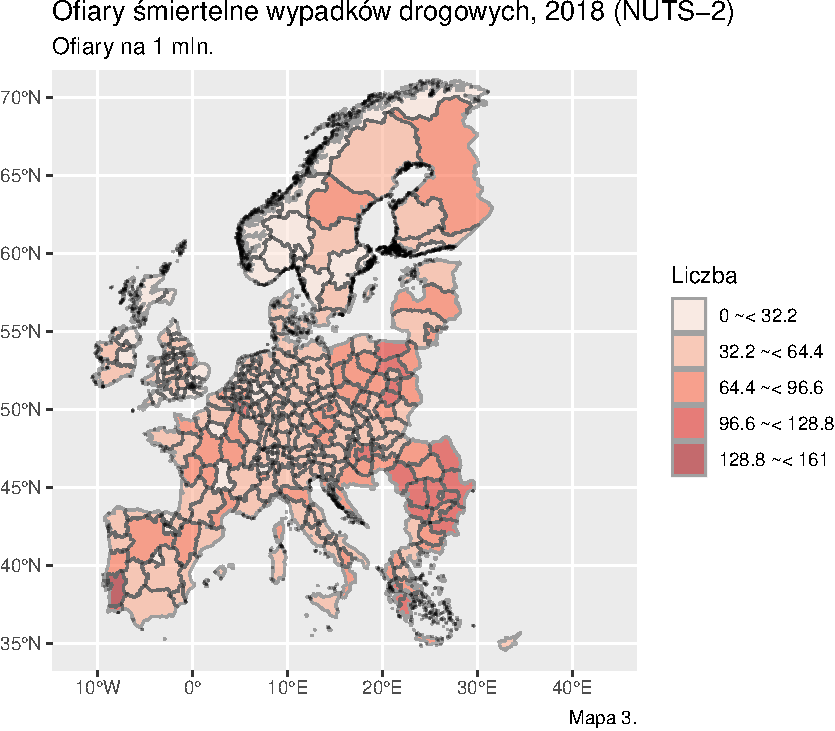
\includegraphics{raport_wypadki_files/figure-latex/unnamed-chunk-23-1} \hfill{}

\caption{Mapa 3.}\label{fig:unnamed-chunk-23}
\end{figure}

Te same dane przestawione na mapie w skali ciągłej.

\begin{figure}

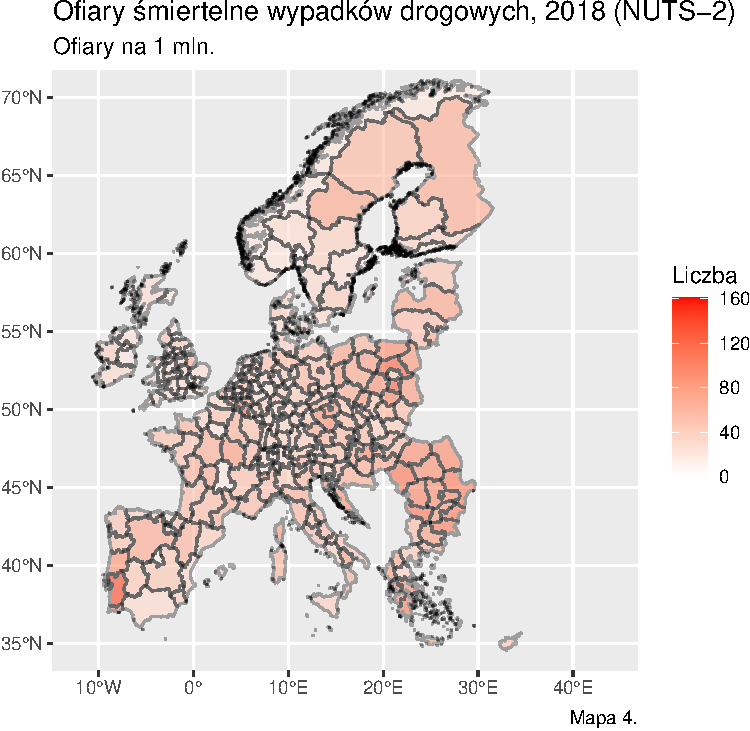
\includegraphics{raport_wypadki_files/figure-latex/unnamed-chunk-24-1} \hfill{}

\caption{Mapa 4.}\label{fig:unnamed-chunk-24}
\end{figure}

Warto w tym miejscu przeanalizować jaka sytuacja pod tym względem
występuje w Niemczech - państwie, które część do 1990 r. znajdowała się
w tzw. Bloku Wschodnim. W tym celu należy przefiltrować dane obejmujące
regiony leżące w obrębie landów niemieckich.

Uzyskane dane zostały przedstawione na mapie Niemiec.

\begin{figure}

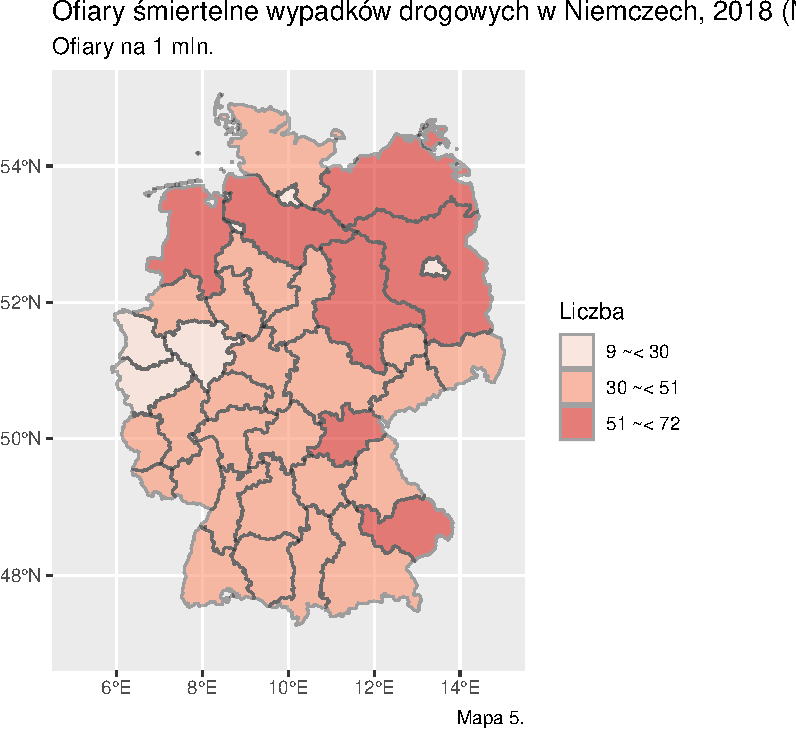
\includegraphics{raport_wypadki_files/figure-latex/unnamed-chunk-26-1} \hfill{}

\caption{Mapa 5.}\label{fig:unnamed-chunk-26}
\end{figure}

Aby lepiej zobrazować w jakim stopniu dane dla obszaru dawnego NRD
różnią się od reszty kraju, należy nałożyć na mapę hsitoryczne granice
Niemiec Wschodnich. W tym celu warto sięgnąć po bibliotekę Cshapes.

Na mapie 6 wyraźnie widać, że problem wysokiej liczby ofiar wypadków
drogowych nie dotyczy wyłącznie obszaru dawnego NRD. Nie zmienia to
jednak faktu, że na tle reszty kraju, niemal cały teb obszar
charakteryzuje sięwysoką liczbą ofiar śmiertelnych będących skutkiem
wypadków drogowych.

\begin{figure}

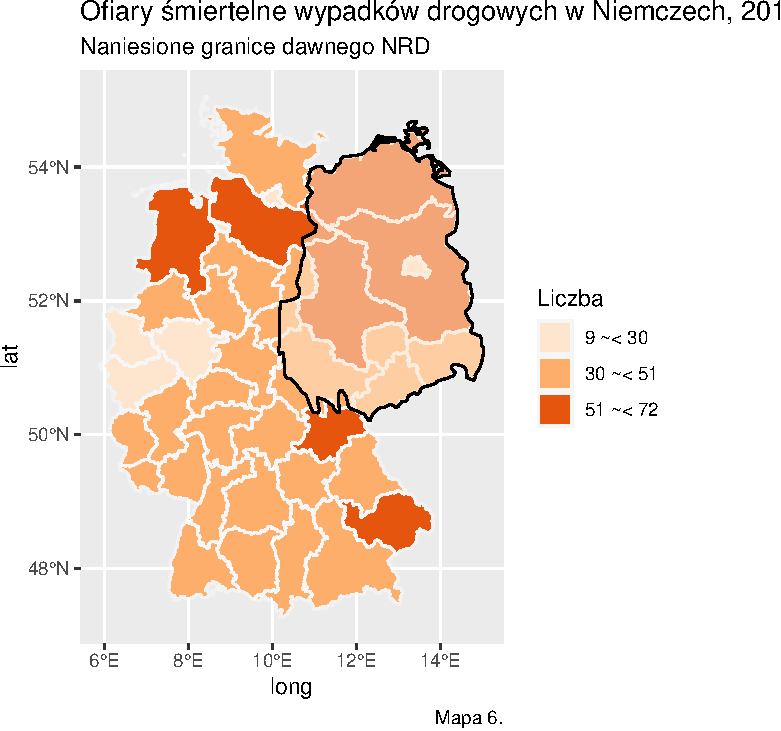
\includegraphics{raport_wypadki_files/figure-latex/unnamed-chunk-28-1} \hfill{}

\caption{Mapa 6.}\label{fig:unnamed-chunk-28}
\end{figure}

Potwierdza to mapa, na której dane przedstawione zostały w skali
ciągłej.

\begin{figure}

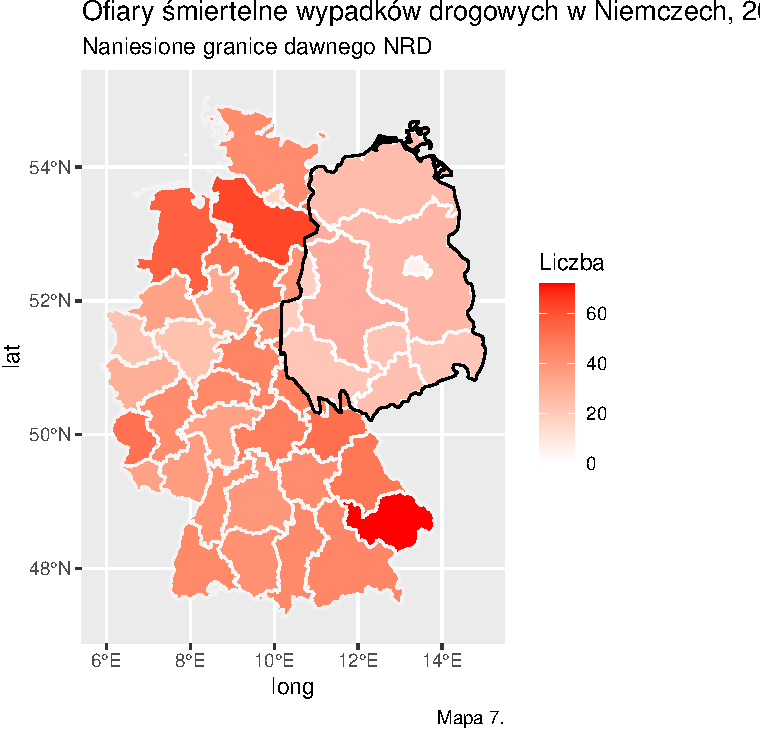
\includegraphics{raport_wypadki_files/figure-latex/unnamed-chunk-29-1} \hfill{}

\caption{Mapa 7.}\label{fig:unnamed-chunk-29}
\end{figure}

\hypertarget{liczba-samochoduxf3w-osobowych-na-1000-mieszkancow}{%
\subsection{liczba samochodów osobowych na 1000
mieszkancow}\label{liczba-samochoduxf3w-osobowych-na-1000-mieszkancow}}

\begin{flushleft}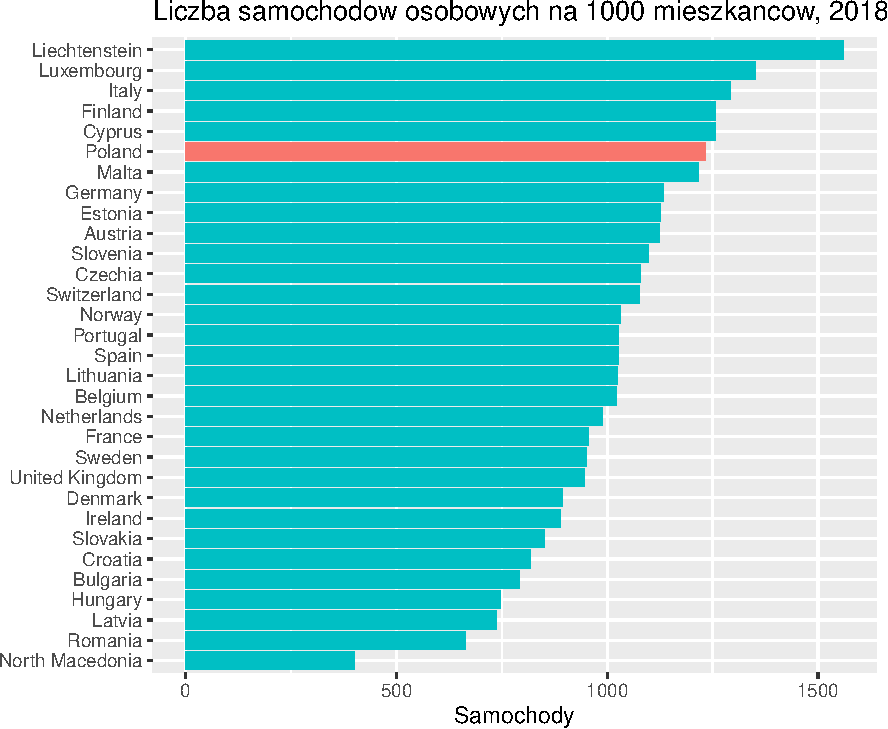
\includegraphics{raport_wypadki_files/figure-latex/unnamed-chunk-31-1} \end{flushleft}

\begin{flushleft}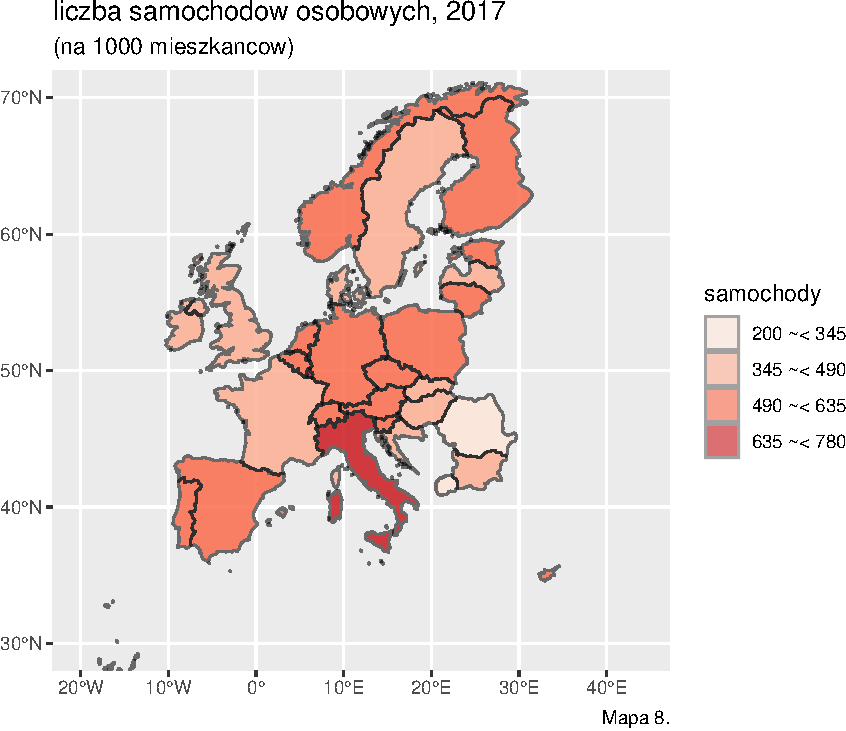
\includegraphics{raport_wypadki_files/figure-latex/unnamed-chunk-31-2} \end{flushleft}

\hypertarget{stosunek-liczby-zgonow-w-wypadkach-drogowych-do-liczby-samochodow}{%
\subsection{stosunek liczby zgonow w wypadkach drogowych do liczby
samochodow}\label{stosunek-liczby-zgonow-w-wypadkach-drogowych-do-liczby-samochodow}}

\begin{flushleft}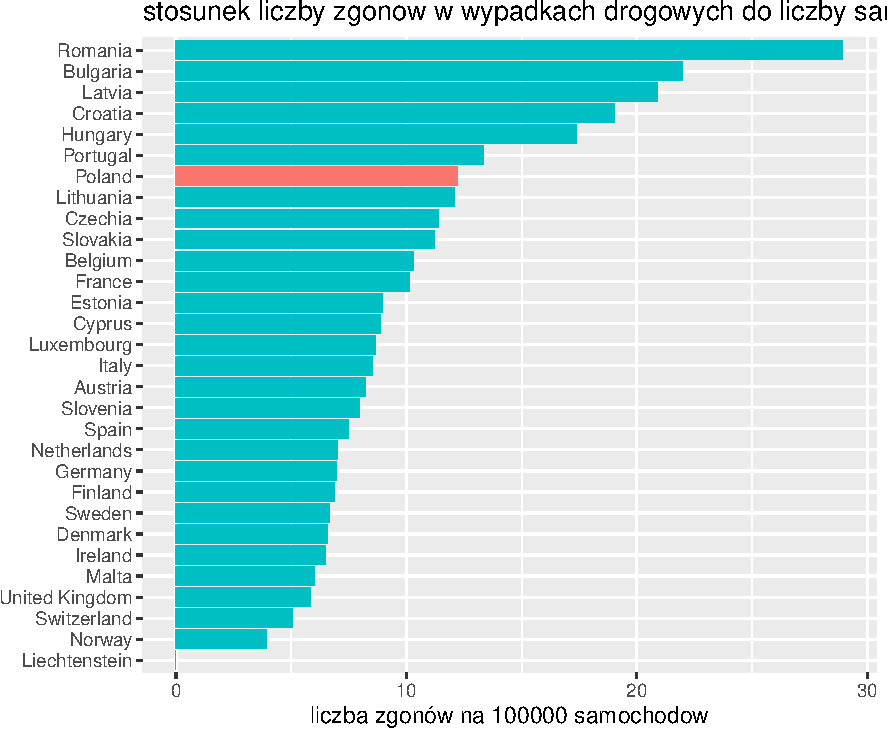
\includegraphics{raport_wypadki_files/figure-latex/unnamed-chunk-33-1} \end{flushleft}

\begin{flushleft}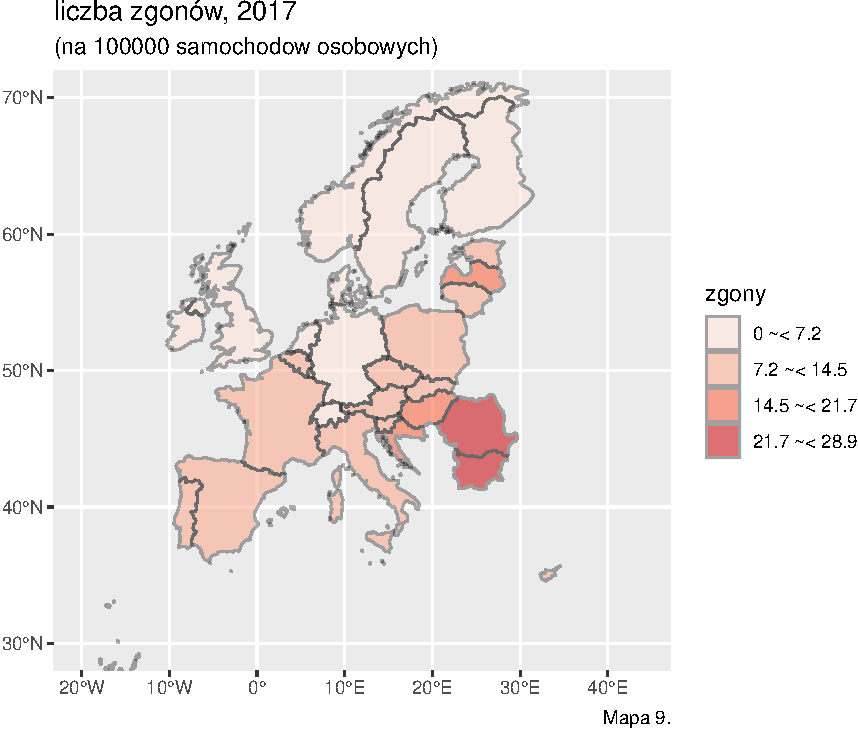
\includegraphics{raport_wypadki_files/figure-latex/unnamed-chunk-33-2} \end{flushleft}

\hypertarget{dane-polska}{%
\section{Dane Polska}\label{dane-polska}}

\hypertarget{analiza-wypadkuxf3w-w-polsce}{%
\subsection{Analiza wypadków w
Polsce}\label{analiza-wypadkuxf3w-w-polsce}}

Na poniższym wykresie porównano zachowanie trendu liczby wypadków
drogowych ze wzrostem kilometrów autostrad w Polsce. Widać, że wraz ze
wzrostem liczby kilometrów oddawanych do użytku autostrad malała liczba
wypadków drogowych.

\begin{flushleft}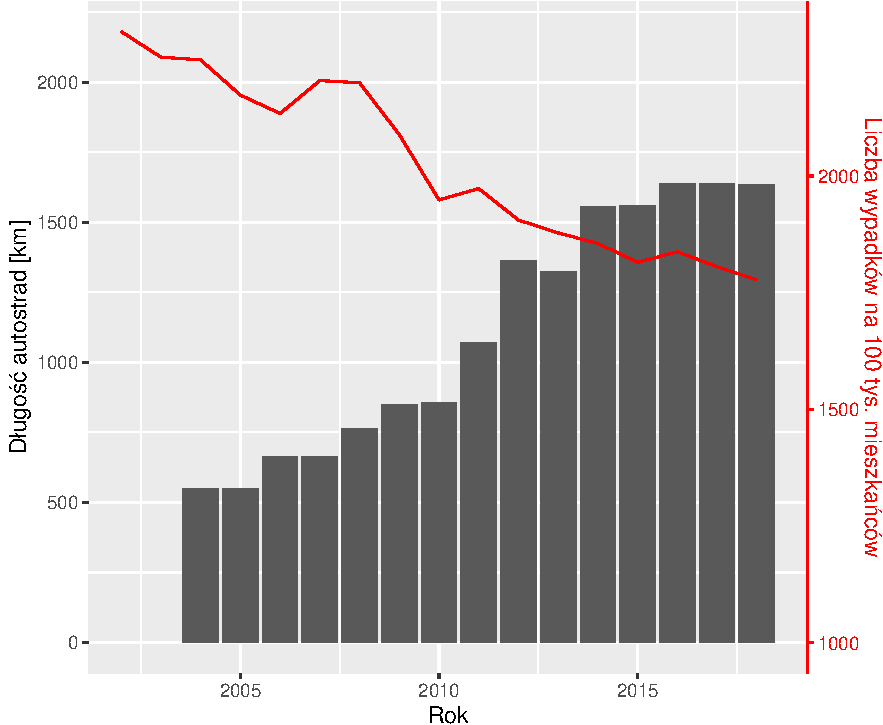
\includegraphics{raport_wypadki_files/figure-latex/pressure-1} \end{flushleft}

\hypertarget{pojazdy-oguxf3ux142em}{%
\subsubsection{Pojazdy ogółem}\label{pojazdy-oguxf3ux142em}}

\begin{verbatim}
## Adding missing grouping variables: `Nazwa`
\end{verbatim}

\begin{flushleft}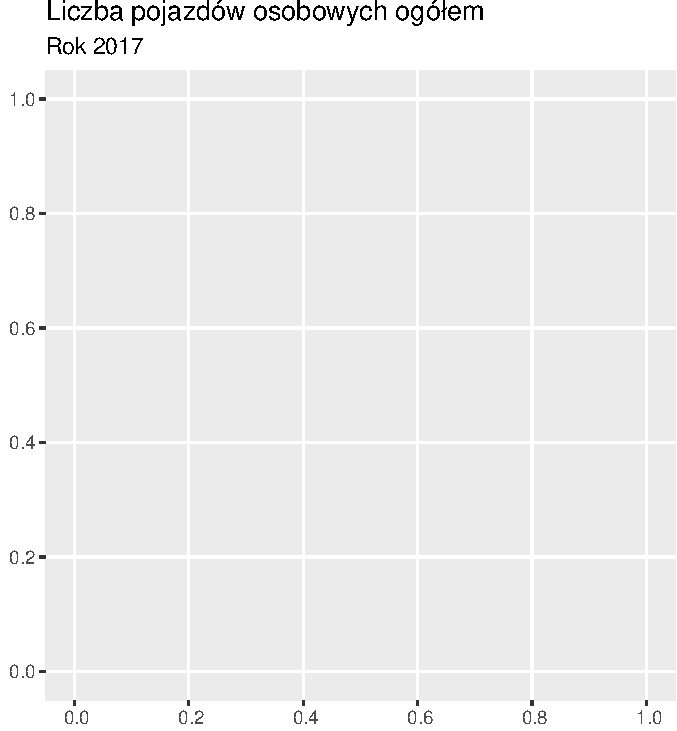
\includegraphics{raport_wypadki_files/figure-latex/pojazdy-1} \end{flushleft}

\hypertarget{pojazdy-na-100-tys.-mieszkaux144cuxf3w-na-mapie}{%
\subsubsection{Pojazdy na 100 tys. mieszkańców na
mapie}\label{pojazdy-na-100-tys.-mieszkaux144cuxf3w-na-mapie}}

\begin{flushleft}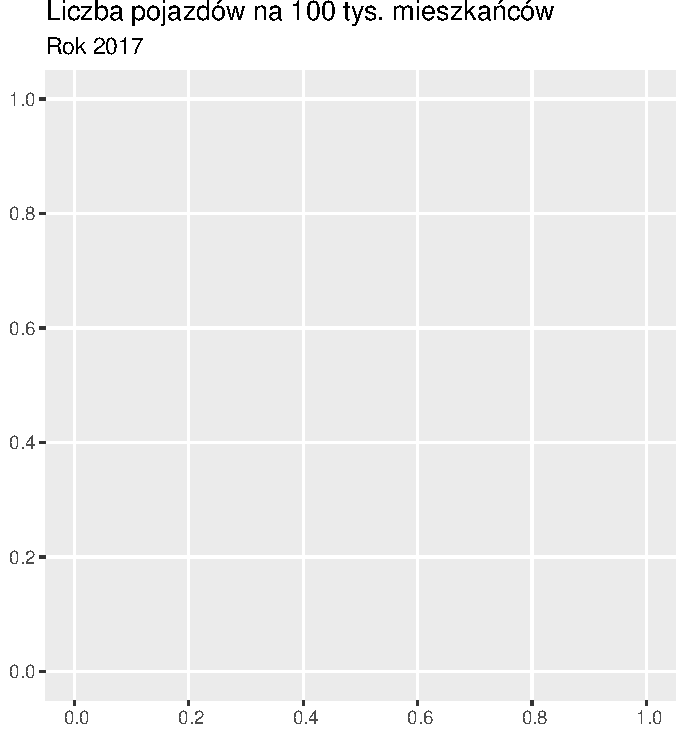
\includegraphics{raport_wypadki_files/figure-latex/unnamed-chunk-34-1} \end{flushleft}

\hypertarget{pojazdy-na-100-tys.-mieszkaux144cuxf3w-na-mapie---klasy}{%
\subsubsection{Pojazdy na 100 tys. mieszkańców na mapie -
klasy}\label{pojazdy-na-100-tys.-mieszkaux144cuxf3w-na-mapie---klasy}}

Na powyższej mapie, liczba pojazdów w powiatach została zobrazowana za
pomocą gradientu koloru. Ze względu na szeroki zakres wartości może być
ciężko odróżnić wartości. Na kolejnej ilustracji wartości podzielono na
zakresy i pokazano 4 klas, które powstały z przedziałów kwantylowych:

\begin{itemize}
\tightlist
\item
  0 - 25 \%
\item
  25 - 50 \%
\item
  50 - 75 \%
\item
  75 - 100 \%
\end{itemize}

\begin{flushleft}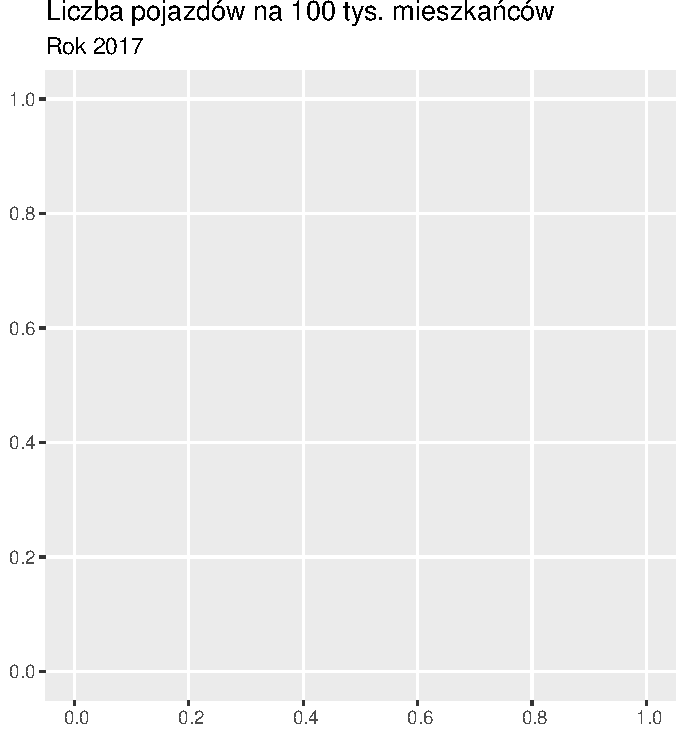
\includegraphics{raport_wypadki_files/figure-latex/unnamed-chunk-35-1} \end{flushleft}

\hypertarget{wykresy-topbottom-10-powiatuxf3w-w-liczbie-zarejestrowanych-auto-osobowych}{%
\subsubsection{Wykresy top/bottom 10 powiatów w liczbie zarejestrowanych
auto
osobowych}\label{wykresy-topbottom-10-powiatuxf3w-w-liczbie-zarejestrowanych-auto-osobowych}}

\begin{verbatim}
## Adding missing grouping variables: `Rok`, `Kod`
\end{verbatim}

\begin{flushleft}
\includegraphics{raport_wypadki_files/figure-latex/unnamed-chunk-36-1} \end{flushleft}

\begin{verbatim}
## Adding missing grouping variables: `Rok`, `Kod`
\end{verbatim}

\begin{flushleft}
\includegraphics{raport_wypadki_files/figure-latex/unnamed-chunk-37-1} \end{flushleft}

\hypertarget{wypadki}{%
\subsection{Wypadki}\label{wypadki}}

\hypertarget{liczba-wypadkuxf3w-na-100-tys.-mieszkaux144cuxf3w-na-mapie-powiatuxf3w}{%
\subsubsection{Liczba wypadków na 100 tys. mieszkańców na mapie
powiatów}\label{liczba-wypadkuxf3w-na-100-tys.-mieszkaux144cuxf3w-na-mapie-powiatuxf3w}}

\begin{flushleft}\includegraphics{raport_wypadki_files/figure-latex/unnamed-chunk-38-1} \end{flushleft}

\hypertarget{wykresy-topbottom}{%
\subsubsection{Wykresy top/bottom}\label{wykresy-topbottom}}

\begin{flushleft}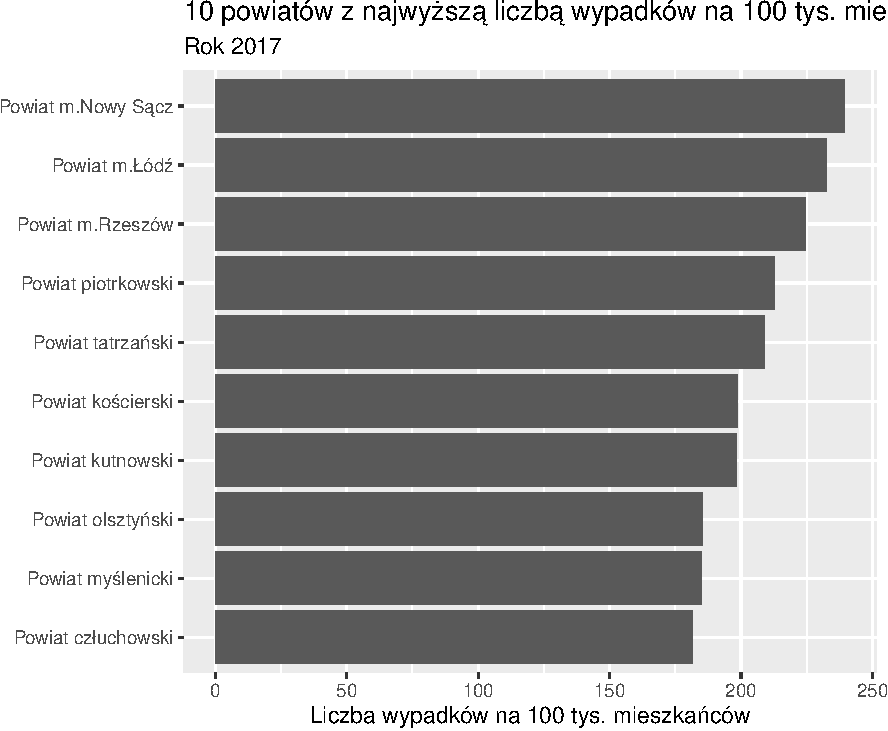
\includegraphics{raport_wypadki_files/figure-latex/unnamed-chunk-39-1} \end{flushleft}

\begin{flushleft}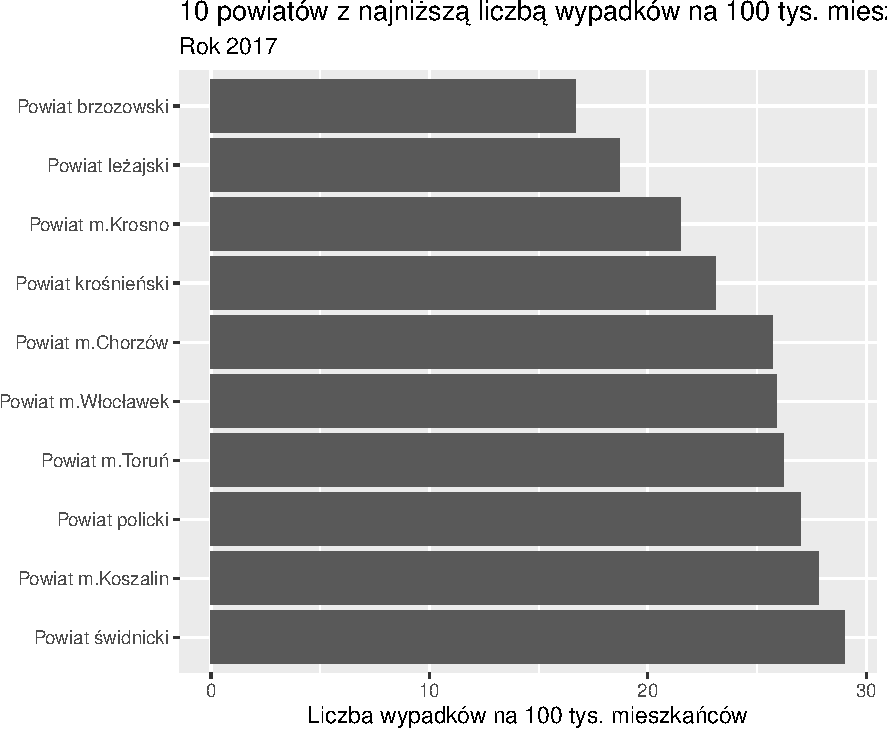
\includegraphics{raport_wypadki_files/figure-latex/unnamed-chunk-40-1} \end{flushleft}

\hypertarget{liczba-ofiar-ux15bmiertelnych-w-wypadkach-na-100-tys.-pojazduxf3w}{%
\subsubsection{Liczba ofiar śmiertelnych w wypadkach na 100 tys.
pojazdów}\label{liczba-ofiar-ux15bmiertelnych-w-wypadkach-na-100-tys.-pojazduxf3w}}

\begin{flushleft}\includegraphics{raport_wypadki_files/figure-latex/unnamed-chunk-41-1} \end{flushleft}

\hypertarget{wykresy-topbottom-1}{%
\subsubsection{Wykresy top/bottom}\label{wykresy-topbottom-1}}

\begin{flushleft}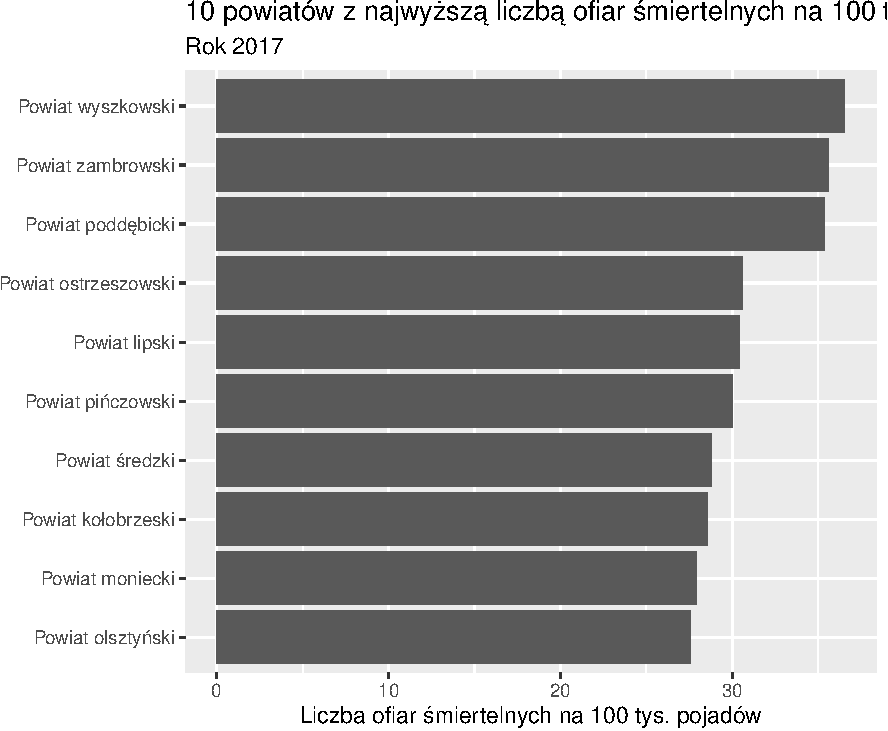
\includegraphics{raport_wypadki_files/figure-latex/unnamed-chunk-42-1} \end{flushleft}

\begin{flushleft}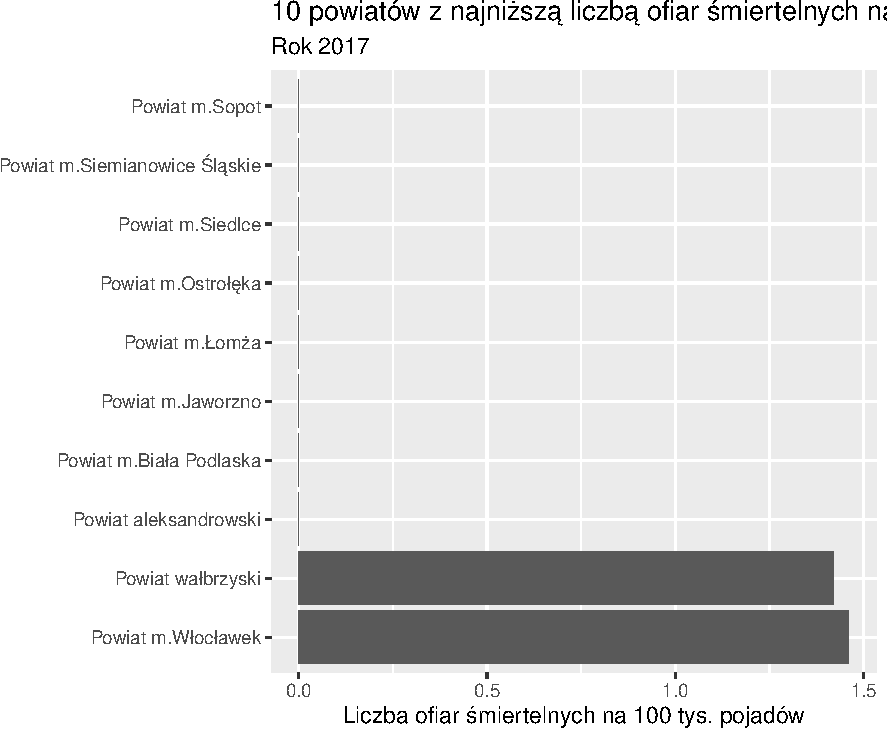
\includegraphics{raport_wypadki_files/figure-latex/unnamed-chunk-43-1} \end{flushleft}

\hypertarget{liczba-ofiar-ux15bmiertelnych-na-100-wypadkuxf3w}{%
\subsubsection{Liczba ofiar śmiertelnych na 100
wypadków}\label{liczba-ofiar-ux15bmiertelnych-na-100-wypadkuxf3w}}

\begin{flushleft}\includegraphics{raport_wypadki_files/figure-latex/unnamed-chunk-44-1} \end{flushleft}

\hypertarget{wykresy-topbottom-2}{%
\subsubsection{WYkresy top/bottom}\label{wykresy-topbottom-2}}

\begin{flushleft}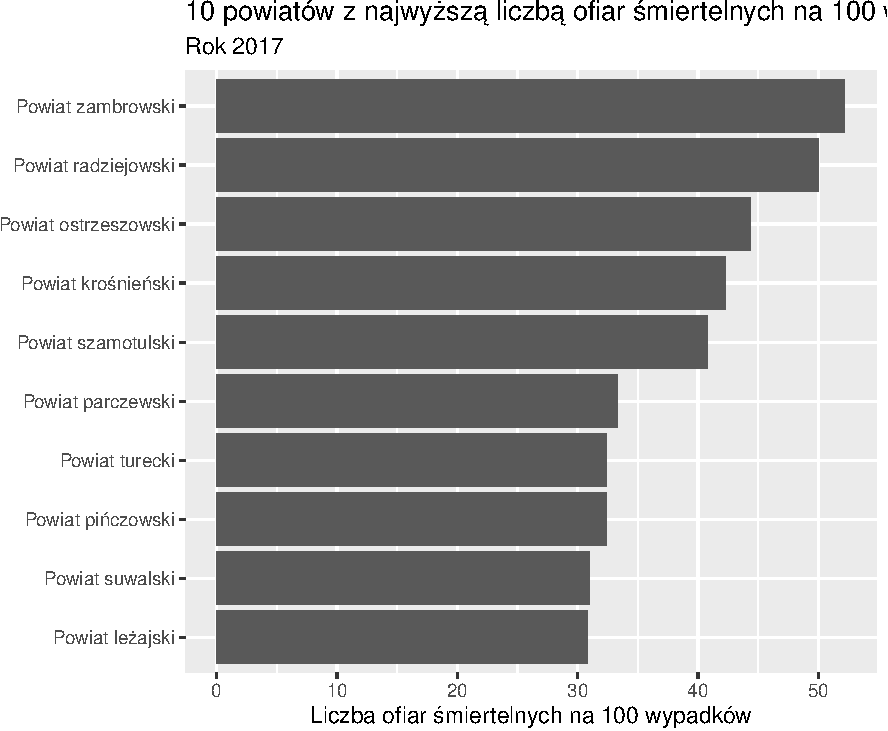
\includegraphics{raport_wypadki_files/figure-latex/unnamed-chunk-45-1} \end{flushleft}

\begin{flushleft}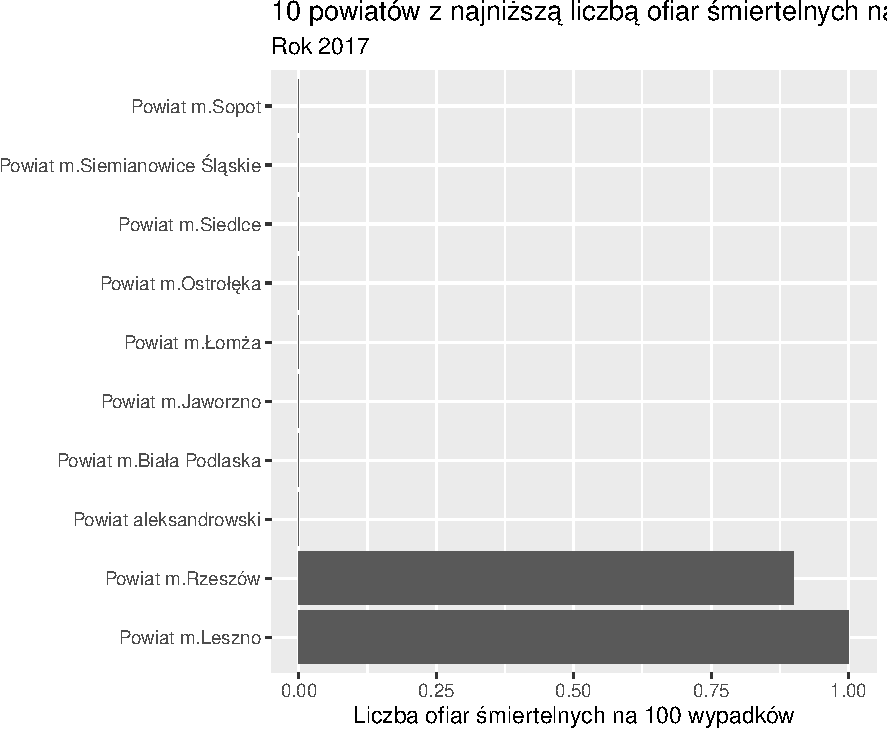
\includegraphics{raport_wypadki_files/figure-latex/unnamed-chunk-46-1} \end{flushleft}

\end{document}
